\paragraph{Introduction: }
Direct Digital Synthesis (DDS) is a method for generating a desired waveform
 (such as a sine wave) by using the technique described in Figure 1 below.

\begin{figure}[htb]
   \begin{center}
      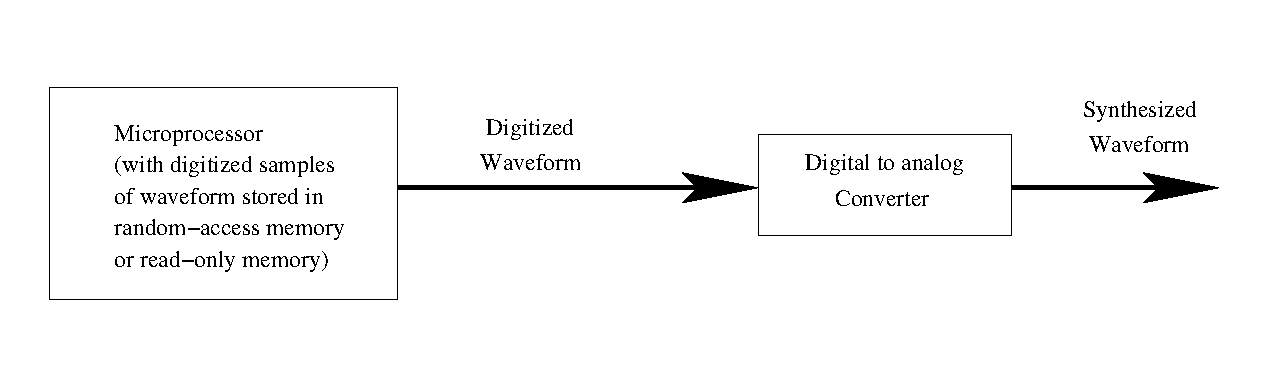
\epsfig{file=fig1.eps,width=14cm}
        \caption{Direct digital synthesis (DDS) [1].}
      \label{fig:fig1}
   \end{center}
\end{figure}

Quantized samples of a desired waveform are stored in the memory of the
 microprocessor system.  This desired waveform can then be generated by
 ``playing out'' the stored words into the digital-to-analog converter.  
The frequency of this waveform is determined simply by how fast the stored 
words are read from memory, and is thus programmable.  Likewise, the phase 
and amplitude of the generated waveform are programmable.

The DDS technique is replacing analog circuits in many applications.  
For example, it is used in higher-priced communication receivers to generate
 local oscillator signals.  It can also be used to generate sounds in 
electronic pipe organs and music synthesizers.  Another application is
 its use by lab instrument manufacturers to generate output waveforms in 
function generators and arbitrary waveform generators [1].

In this lab you will familiarize yourself with the capabilities of the
 Analog Devices AD9854 DDS.  The DDS board is installed between the 
6-channel card and the DSP card at some (not all) lab stations.  You can tell which boxes have them 
by the way the 6-channel card sits higher inside the metal box.


\section{Frequency Modulation (FM) Radio Exercise}
To get your feet wet and see a demonstration 
of the DDS, perform the following exercise.  
Copy the files \verb+FM.asm+ and \verb+core_mod.asm+ from the 
\verb+v:\ece320\54x\dds\+ directory.  Assemble
 and run the frequency modulation (FM) program
 \verb+FM.asm+.  Next, plug an audio source into one 
of the two DSP input channels that you've been
 using all semester.  If you have a CD on you, 
pop it into the computer and use that.  If not, 
use a music web site on the Internet as your 
audio source.  Connect the computer 
to the DSP by using a male-male 
audio cable and an audio-to-BNC converter box 
(little blue box), both of which are in the lab.  
The computer has three audio outputs on the back; 
use the middle jack.  Ask your TA if you can't 
find the cable and/or box or don't see how to 
make the connection.  Next, connect a dipole antenna 
to the output of the DDS (port \#1 on the back of the DDS board). 
 A crude but effective dipole antenna can be formed
 by connecting together a few BNC and banana cables in the shape of a \verb+T+.  
There should be one or two of these concoctions in the lab.  
Once the connections are made, turn on the black 
receiver in the lab, and tune it to 104.9 MHz 
(wide band FM).  You should be able to hear your 
audio source!  NOTE: If your audio sounds distorted, 
it's most likely due to the volume of your audio 
source being too loud and getting clipped by 
the DSP analog-to-digital converter.

  
\paragraph{Spectral Copies: }The digital-to-analog converter on the DDS is 
unfiltered, which means that there is no anti-imaging filter to 
remove the spectral replicas.  To see this, plug the output of the DDS board 
directly into the vector signal analyzer (VSA), and observe the spectrum.  Use 104.9 MHz as the center
 frequency, and set the span wide enough so that you can see the spectra of the
 replicas to the left and right of the 104.9 MHz signal.  Use the marker to find
 the peaks of the other replicas, and record their frequencies.  Once you've done 
that, reattach the antenna to the DDS output, and tune the receiver to the frequencies
 you just recorded.  You should be able to hear your audio on each of the other 
frequencies.  Note: The clock rate of the DDS is 60MHz, which corresponds to $2\pi$ 
in digital frequency.  Therefore, the 104.9 MHz signal you just 
listened to is roughly equivalent to $7\pi/2$ in digital frequency.  
What are the digital frequencies of the other copies you saw on the VSA? 

\section{How to use the DDS}
The DDS has several different modes of operation: single-tone, unramped Frequency 
Shift Keying (FSK), ramped FSK, chirp, and Binary Phase Shift Keying (BPSK).  In
 this lab we will use the DDS in single-tone mode.  Single-tone mode is easy to use, 
and is powerful enough to create many different kinds of waveforms, including FM and FSK.

\subsection{FM code}
The FM code you just ran (also listed in the Appendix) is fairly straightforward.  
The program first calls the \verb+radioinit+ subroutine.  This routine sets the DDS
 to single-tone mode and turns off an inverse-sinc filter to conserve power. 
 Following \verb+radioinit+, the \verb+setcarrier+ subroutine is called.  This routine sets the 
frequency of the DDS output by writing to the two most significant 8-bit frequency 
registers of the 48-bit frequency-tuning word on the DDS (Communication between the DSP and 
the DDS is done through a parallel bus).  Although the frequency-tuning word on the DDS 
has 48 bits of resolution, the upper 16 bits provide us with enough resolution for the 
purposes of this lab, and so we will only be writing to the two most significant registers.  
See page 26 in the DDS data sheet for a layout of the frequency-tuning word.  

To set the carrier frequency, we first need to determine what frequency word has 
to be written to the frequency registers on the DDS.  This can be done using equation 1:
\begin{equation}
\mbox{Frequency word}=\frac{\mbox{baseband frequency}}{60 MHz}2^{48}
\end{equation}
where "baseband frequency" corresponds to the desired frequency that lies in the range 
of 0-30 MHz.  For example, to get the DDS to transmit at 104.9 MHz, you would choose 
the baseband frequency to be 15.1 MHz since 104.9 MHz is one of the unfiltered spectral replicas of 15.1 MHz. 
 Then, using the equation, the frequency word for 15.1 MHz (and 104.9 MHz) would be equal 
to 406D 3A06 D3D4h.  But since we only write to the two most significant registers of the 
frequency-tuning word, we only need the first 4 hexadecimal numbers of this result, i.e. 406Dh.  
The first two of those, 40h, need to get written to the most significant 8-bit frequency 
register, while the second two hex numbers, 6Dh, need to get written to the second-most 
significant 8-bit frequency register.  This is where the 40h and 6Dh in the \verb+setcarrier+ 
subroutine of the FM code come from.  

Writing to the frequency registers is accomplished using the \verb+portw+ instruction.  To write
 to the frequency or phase registers on the DDS, the second operand of the \verb+portw+ instruction
 must be 10xxxxxx, where the lower six bits are the address of the specific register to be 
written to.  The address of the most significant frequency register on the DDS is 04h, and 
the address of the second most significant frequency register on the DDS is 05h (see page 26 
in the data sheet).  It is important to note that the way our DDS boards were built, you will not 
be allowed to make two consecutive writes.  To solve this problem, a subroutine called 
\verb+nullop+ is called to waste some CPU time between writes.  \verb+nullop+ does this by simply repeating 
the 'nop' instruction 128 times.  

After the program returns from the \verb+setcarrier+ subroutine, it enters an infinite loop in which 
it waits for a serial interrupt to occur.  The serial interrupt occurs every time a 
new sample is acquired from one of the two input channels and is transmitted to the DSP via the serial port.  
When the interrupt occurs, an interrupt service routine called \verb+ANALOG_IFC+ 
(see \verb+core_mod.asm+) executes and calls the \verb+handle_sample+ subroutine.  The 
\verb+handle_sample+ subroutine 
reads in the acquired sample from the serial port and scales that sample so that it can
 be "mapped" to a frequency in the range of $\pm$75 kHz (In FM radio, the amplitude of the message 
signal being transmitted determines the amount of frequency deviation from the carrier frequency 
of the passband signal.  $\pm$75 kHz is the largest frequency deviation allowed).  The scaled sample 
therefore determines the frequency deviation, and is added to 6Dh.  The last step is to write the 
result to the second most significant frequency register so that the frequency of the DDS output 
can be updated.       

\subsection{Programming the Phase}
The process for changing the phase of the DDS output is the same as it was for changing the 
frequency of the DDS output.  To change the phase, you need to write a phase word to a phase-adjust
 register on the DDS.  The phase-adjust register is 14 bits wide and is split up into
 two smaller registers that you can write to (see page 26 in the data sheet).  The upper 6 bits 
have address 00h, and the lower 8 bits have address 01h.  The phase word can be calculated 
using equation 2:

\begin{equation}
\mbox{Phase word} =\frac{\mbox{Carrier phase}}{2\pi}2^{14}
\end{equation}

Once you've calculated the phase word, you can write it to the DDS using the \verb+portw+ 
instruction as before.  Just make sure you use the correct address for the phase register.

\subsection{Programming the Amplitude}  
The DDS also allows you to program the amplitude, but this functionality is not addressed 
in this lab.  You will be able to implement a digital communication system in ECE320 
without having to program the amplitude.  Interested readers are referred to the data sheet.

\section{FSK exercise}
Now that you know how to use the DDS in single-tone mode, implement a simple FSK system that 
uses 2 frequencies: 120.005 MHz, and 120.011 MHz.  You don't need to encode any data for this 
exercise.  In other words, your DDS output should just continuously alternate between the two 
frequency symbols.  Also, the DDS automatically ensures continuous phase, so you won't have to 
keep track of it.  Use a symbol length of approximately 725$\mu$s (the same length as your lab 5 
symbols).  Timer interrupts are an elegant way to control the symbol lengths, but in this lab
 we will keep things simple and control the symbol lengths by creating a second (longer) nullop 
subroutine and calling it between writes to the DDS.  The second nullop subroutine should waste 
approximately 725$\mu$s worth of time.  Note: since we're not using input or output from the DSP, 
you don't need to use the WaitData or WaitAudio macros.  

\subsection{Testing}
Note that the corresponding baseband frequencies for 120.005 MHz and 120.011 MHz are 5 kHz, and 
11 kHz, respectively.  Since these baseband frequencies lie within the 22.05 kHz bandwidth of 
the DSP, you will be able to view your FSK signal in real time on the oscilloscope {\bf without} the 
contribution from the spectral replicas.  Just feed the output of the DDS into a second DSP (the anti-aliasing
filter on the DSP will get rid of the spectral replicas), and 
pass it through to the output and the scope.  You should be able to verify that there is continuous 
phase between frequency symbols, and that your symbol length is approximately 725$\mu$s.  You should 
also view the spectrum of your DDS output on the VSA to verify that your symbols have 
the correct frequencies.

\newpage
{\bf References} \\ 

[1] Leon W. Couch II. Digital and Analog Communication Systems.  Prentice Hall, Upper \\ 
Saddle River, New Jersey, 07458.

\newpage
{\bf Appendix: FM.asm}
\setlength{\baselineskip}{0.4cm}
\listinginput{1}{FM.asm}
\setlength{\baselineskip}{0.5cm}

